\documentclass[review]{elsarticle}
% for submission use preprint
% review for

\usepackage{lineno,hyperref}
\usepackage{amsmath}
\modulolinenumbers[5]

\journal{Journal of Networks and Computer Applications}

%%%%%%%%%%%%%%%%%%%%%%%
%% Elsevier bibliography styles
%%%%%%%%%%%%%%%%%%%%%%%
%% To change the style, put a % in front of the second line of the current style and
%% remove the % from the second line of the style you would like to use.
%%%%%%%%%%%%%%%%%%%%%%%

%% Numbered
%\bibliographystyle{model1-num-names}

%% Numbered without titles
%\bibliographystyle{model1a-num-names}

%% Harvard
%\bibliographystyle{model2-names.bst}\biboptions{authoryear}

%% Vancouver numbered
%\usepackage{numcompress}\bibliographystyle{model3-num-names}

%% Vancouver name/year
%\usepackage{numcompress}\bibliographystyle{model4-names}\biboptions{authoryear}

%% APA style
%\bibliographystyle{model5-names}\biboptions{authoryear}

%% AMA style
%\usepackage{numcompress}\bibliographystyle{model6-num-names}

%% `Elsevier LaTeX' style
\bibliographystyle{elsarticle-num}
%%%%%%%%%%%%%%%%%%%%%%%

\begin{document}

\begin{frontmatter}

\title{A wearable fall-detection system based on Body Area Networks for smart cities}

%% Group authors per affiliation:
\author{Luigi La Blunda\fnref{label1}}
\ead{l.lablunda@fb2.fra-uas.de (corresponding author)}
\author{Lorena Guti\'errez-Madro\~nal\fnref{label2}}
%% \author{Name\corref{cor1}\fnref{label2}}
\ead{lorena.gutierrez@uca.es}
\author{Matthias F. Wagner\fnref{label1}}
\ead{mfwagner@fb2.fra-uas.de}
\author{I. Medina-Bulo\fnref{label2}}
\ead{inmaculada.medina@uca.es}
\address[label1]{WSN and IOT Research Group Frankfurt University of Applied Sciences, Nibelungenplatz 1, 60318 Frankfurt am Main, Germany}
\address[label2]{UCASE Software Engineering Research group, University of Cadiz}



%% or include affiliations in footnotes:
%\author[mymainaddress,mysecondaryaddress]{Elsevier Inc}
%\ead[url]{www.elsevier.com}
%
%\author[mysecondaryaddress]{Global Customer Service\corref{mycorrespondingauthor}}
%\cortext[mycorrespondingauthor]{Corresponding author}
%\ead{support@elsevier.com}
%
%\address[mymainaddress]{1600 John F Kennedy Boulevard, Philadelphia}
%\address[mysecondaryaddress]{360 Park Avenue South, New York}

\begin{abstract}
Falls can have serious consequences for people, which can lead, for example, to restrictions in mobility or in the worst case to traumatic based cases of death. To provide rapid assistance, a portable fall detection system has been developed which is capable of detecting fall situations and, if necessary, alerting the emergency services without any user interaction. The prototype was designed to facilitate a reliable fall-detection and to classify several fall-types. This solution represents a life-saving service for every inhabitant which would significantly enrich the development of smart cities and smart factories where fall-events are part of daily-life. This paper will also introduce the fall analysis, which includes the generation of test events. To guarantee functional safety, the hazard analysis method STAMP (System-Theroetic Accident Model and Processes) will be applied. 
\end{abstract}

\begin{keyword}
e-Health \sep fall-detection\sep Body Area Network \sep safety \sep STAMP \sep Smart City \ 
\end{keyword}

\end{frontmatter}

%\linenumbers

\section{Introduction}
Fall-detection is gaining in importance not only in aging societies, but also in working society and in daily activities. According to the World Health Organization (WHO), 646,000 fatal falls are estimated to be the second leading cause of accidental or unintentional death worldwide each year. People over 65 suffer the most fatal falls. Another high risk group is children. Taking into consideration their evolving developmental stages, the increasing curiosity to explore the environment or the inadequate adult supervision lead to fall-events \cite{WHO2018}.
In everyday life we are also confronted with risk of falling. Working in hazardous working conditions is another risk factor for causing fall-events. An exemplary event could be a worker that falls during the night shift in the factory and no one is there to provide prompt assistance. Another example could be a technician which falls from height while maintaining windmills. Mostly windmills are installed in uninhabited areas where no immediate rescue measures can be taken. Considering these events the consequences can be fatal for the affected people. 
The World Health Organization stated that annually 37.3 million fall-events are severe enough to require medical treatment \cite{WHO2018}. Fall-events leads to the side effects of physical inactivity and loss of balance, especially among old people. Elderly people are scared to fall again and this uncertainty of movement increases the risk of repeated falls. 
To counteract these life-threatening events fast assistance is necessary due to the fact that an unconscious person may not be able to call the emergency services. An approach could be the continuous tracing of medical and / or physical parameters via a wearable sensor network (see Figure \ref{fig:escalationscheme}).
\begin{figure}[!ht]
	\centering
	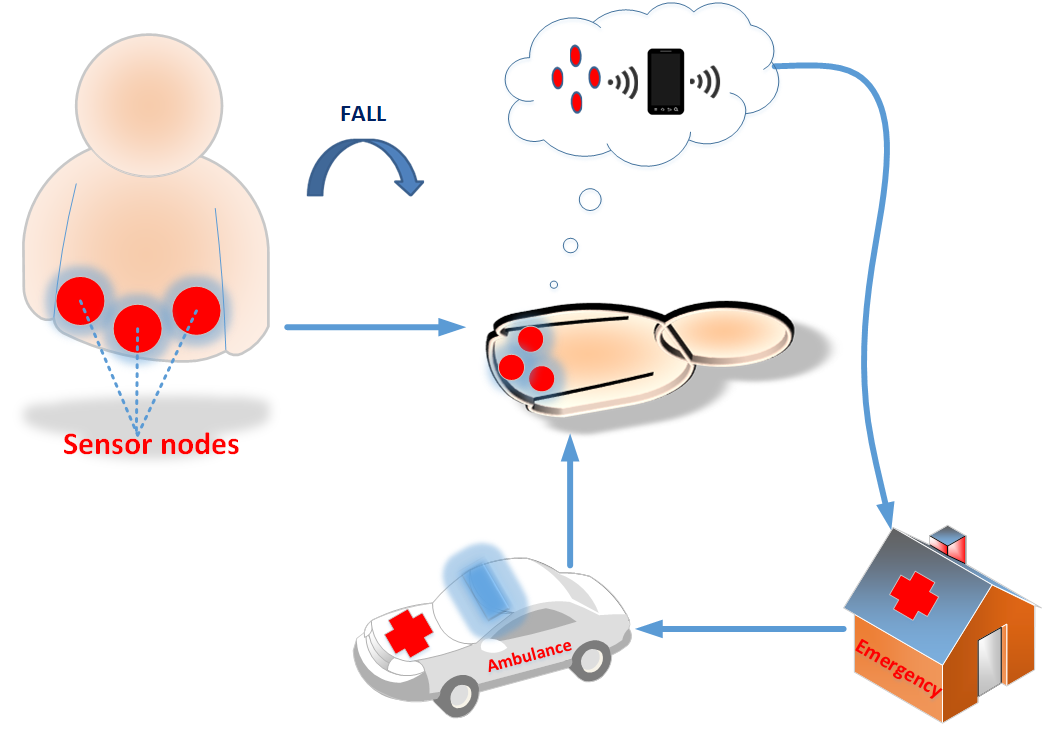
\includegraphics[scale=0.35]{Images/EscalationScheme}
	\caption[Escalation scheme]{Escalation scheme simulation~\cite{LaBlunda.2016,LaBlunda.2016b}}
	\label{fig:escalationscheme}
\end{figure}
A prototype in form of a belt was developed which includes an Electrocardiogram (ECG) - harness and is based on a five sensor nodes Body Area Network (BAN). Each sensor node of the belt acquires continuously acceleration data including time stamp and the sensor node of the ECG-harness provides the analog value of the voltage including time stamp. In case of a fall the system should be capable to autonomously call the emergency services. Applying sensor fusion of physical and medical sensors we expect to improve the reliability of fall-detection and possibly fall-prevention. Another expectation is that the integration of medical sensors may facilitate the classification of different fall-types. In terms of smart cities our expectancy is to significantly provide an important e-health service for smart cities which is an essential life-saver for the population.

The paper is structured as follows. Section \ref{sec:relatedwork} describes the related work regarding fall-detection. In this section a short overview about existing solutions and different approaches for fall-detection is given. Section \ref{sec:background} will describe the basic principles on which our ongoing fall-detection research is based. In the successive section (Section \ref{sec:fall-detectionPrototype}) a detailed description of the fall-detection prototype, including the usage of the ECG-sensor are introduced. Additionally, this section contains the generation of test events which includes the results of the fall-analysis and detected problems. Section \ref{sec:STAMP} will introduce the Hazard analysis method STAMP which is applied on the fall-detection prototype.
Finally, in section \ref{sec:conclusion} a conclusion about this ongoing research is given, including some indications for improvement which could be applied in the future work.

\section{Related Work}
\label{sec:relatedwork}
In this section an overview about several fall-detection approaches is given. There are several techniques which can be applied to detect fall-events. Igual et al. \cite{Igual2013} illustrates the following different types of fall-detection  systems:
\begin{itemize}
	\item Context-aware systems
	\item Wearable systems
\end{itemize}
The functionality of context-aware systems depends on the environment, since the sensors and actuators must be installed in the living area (apartment, nursing home) in order to detect possible fall situations. The video-based context-aware solutions have the advantage to provide an accurate and reliable detection of falls with a fast assistance, but these systems have an issue regarding privacy. Patients using this solution are non-stop monitored and this is not well accepted by many. Additionally, the high purchase price is an obstacle for many patients and the dependency on the environment makes this approach useless, because it would not detect fall-events happening outside the networked area.

The other category of fall-detection systems analyzed by Igual et al. \cite{Igual2013} contains wearable solutions worn on the body and are based on Body Area Networks (BAN). This solution is capable to provide a fall-detection which is independent from the environment in contrast to context-aware systems. The analysis of Igual et al. \cite{Igual2013} illustrates wearable fall-detection systems using the sensor fusion method which comprises accelerometer and gyroscope data and built-in systems in form of smart phone sensors. For both categories of fall-detection solutions (context-aware \& wearable solution) several techniques were used. The following methods were applied for context-aware systems:
\begin{itemize}
	\item Image processing and threshold-based recognition
	\item Image processing and classification models
\end{itemize}
The techniques used for the fall-detection in wearable solutions are the following:
\begin{itemize}
	\item Threshold-based approach
	\item Fall-detection based on machine learning
\end{itemize}
Taking into consideration the fact that it is an essential advantage to focus on wearable solution because of the system's functional independence the scientific work of Li et al. \cite{Li2009} will be explained subsequently. The solution of Li et al. \cite{Li2009} includes two wearable sensor nodes which are based on a BAN. These sensor nodes consist of an accelerometer and gyroscope and they are placed on the chest (Node A) and on the thigh (Node B, see Figure \ref{fig:LietAl-Architecture}). 
\begin{figure}[!ht]
	\centering
	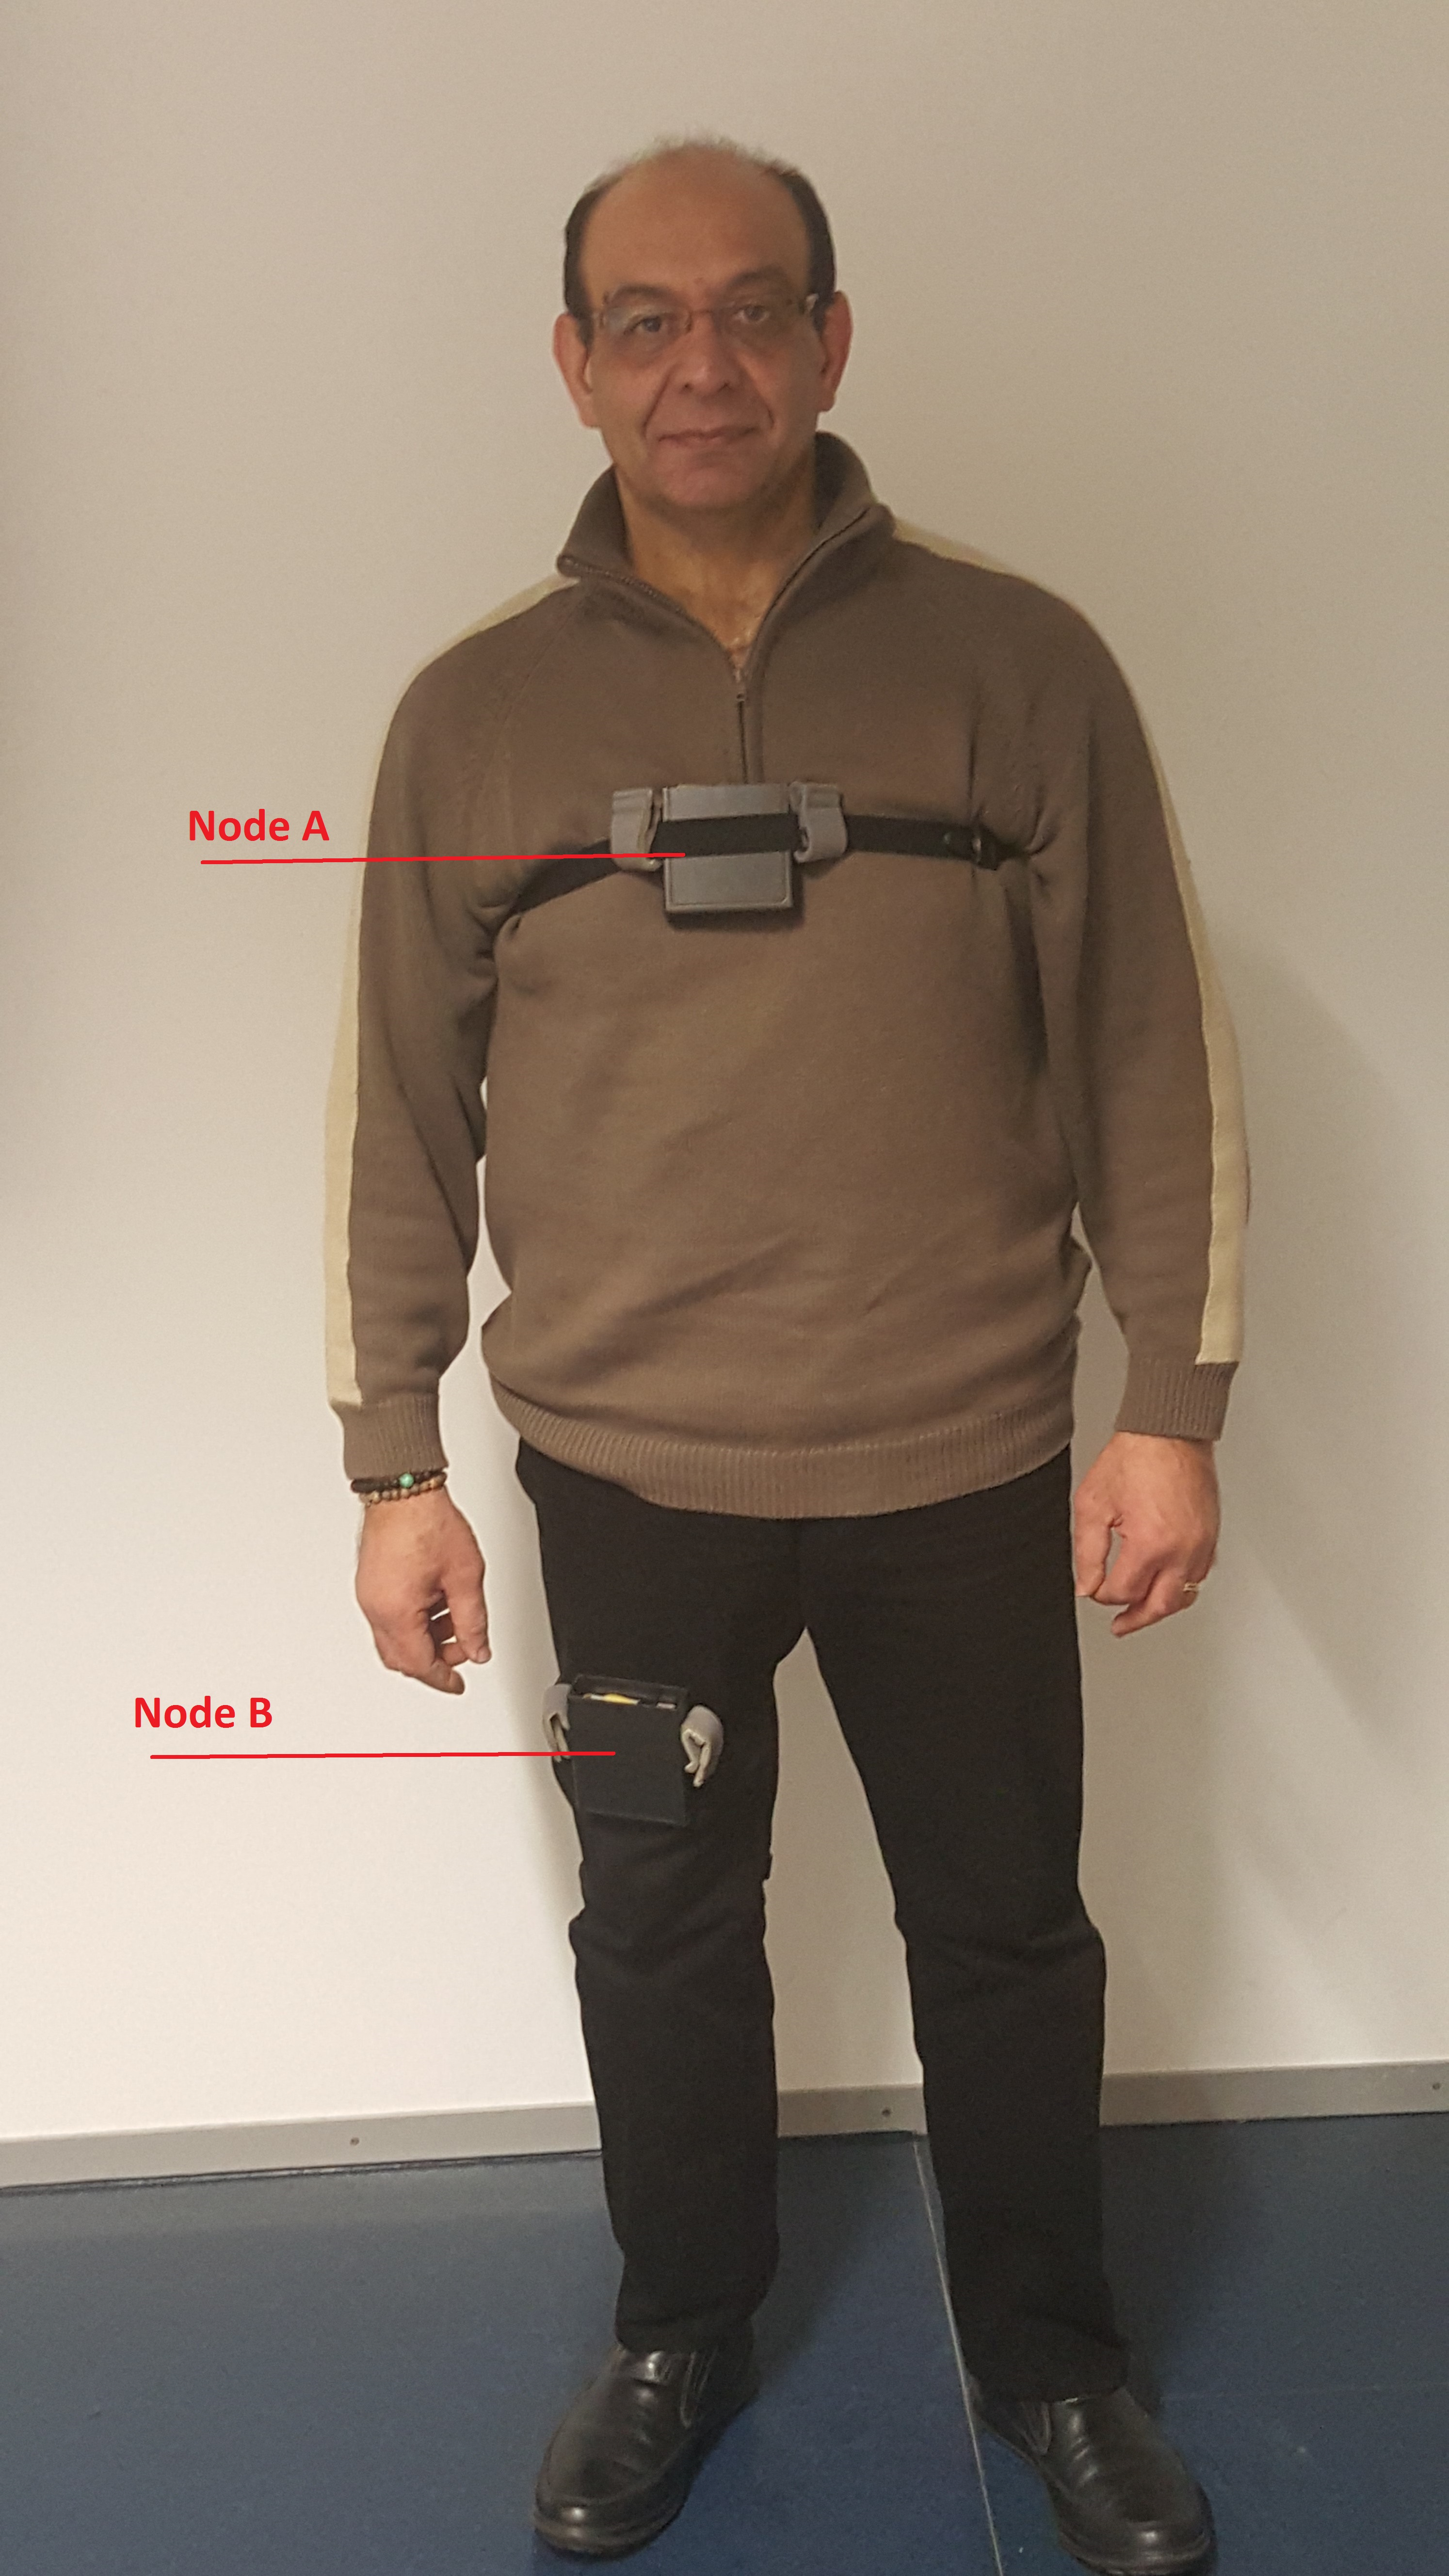
\includegraphics[scale=0.06]{Images/Stankovic_papa2}
	\caption[System architecture according to Li et al.]{System architecture according to Li et al. \cite{Li2009}}
	\label{fig:LietAl-Architecture}
\end{figure}
Li et al. distinguish between two different motion sequences which are used for activity categorization:
\begin{itemize}
	\item Static postures:
	\begin{itemize}
		\item Standing, sitting, lying
	\end{itemize}
	\item Dynamic postures:
	\begin{itemize}
		\item Activities of daily life (ADL) $\rightarrow$ walking, go up / down stairs, sit, jump, lay down, run
		\item Fall-like motions $\rightarrow$ quick sit-down upright, quick sit-down reclined
		\item Flat surface falls $\rightarrow$ fall forward, fall backward, fall right, fall left
		\item Inclined falls $\rightarrow$ fall on stairs
	\end{itemize}
\end{itemize}
A 3-phase Algorithm for fall-detection is proposed by Li et al. to decrease the computational effort of the micro controller. The first phase of the fall-detection algorithm examines if the person is in a static or dynamic position. If the analyzed position coincides with a static postures in the second phase it will be checked whether it corresponds to lying. If lying position, it will be checked if the transition to this posture was intentional or unintentional (3.Phase). To determine it, the previous 5 seconds of data is used. In the case it was unintentional the event will be classified as a fall. The proposed approach in \cite{Li2009} uses a threshold based technique that is applied in the different phases of the algorithm. The weakness of this approach is to differentiate between jumping into bed and falling against wall with seated posture. Collado Villaverde et al. \cite{colladomachine} propose a wearable fall-detection solution based on a smartwatch using acceleration data in combination with machine learning techniques.

A different approach to detect fall-events is presented by Lüder et al. \cite{Luder2009} which apply an air pressure sensor in addition to the accelerometer. The minor air pressure changes correspond to an altitude change of 25 cm which is a relevant indication in combination with accelerometer data of a possible fall-event.  This sensor combination is incorporated in the hardware "StairMaster" of the Frauenhofer Institute. The hardware architecture proposed in \cite{Luder2009} depicts a wearable solution which is worn on the hip and provides wireless data transmission via Bluetooth. Alternatively, the data can be stored on a Secure Digital (SD) card for evaluation purposes. Due to the fact that air pressure can be influenced by meteorological disturbances Lüder et al. \cite{Luder2009} introduced an alternative architecture. This alternative approach incorporates an external barometric sensor as a reference, which is placed in a stationary altitude to compare both air pressure data (wearable \& stationary). Another method for fall-detection based on sensor fusion techniques is described by Gjoreski et al. \cite{Gjoreski2014}. Accelerometer and electrocardiogram (ECG) data is used to detect fall-events. The solution in \cite{Gjoreski2014} is capable of identifying person's movements and fall-situations using wearable sensor nodes based on Bluetooth. These nodes are placed on the chest and thigh which is similar to Li et al's \cite{Li2009} approach. The advantage of the proposed solution by Gjoreski et al. \cite{Gjoreski2014} is the integration of medical sensors. The fusion of acceleration data and ECG-Signal facilitates the detection of anomalies in person's behavior and heart related problems that my lead to falls. The results presented in \cite{Gjoreski2014} emphasize that the incorporation of the ECG-signal can significantly increase the system's reliability to detect fall-events. According to the analysis of Gjoreski et al. \cite{Gjoreski2014} differences in the ECG-signal in different postures were detected. Lower beat rates in the static positions lying and sitting compared to waling were determined. Comparing the beat rates of both static postures (lying and sitting) differences were observed, where the beat rate of lying is lower than the one of sitting.



\section{Background}
\label{sec:background}
The fall-detection prototype is based on the approach proposed in \cite{Gjoreski2014, Kozina}. To detect a fall-event a typical physical behavior is used which comprises the following the phases (see Figure \ref{fig:fallKozina}):
\begin{itemize}
	\item Pre-fall-phase 
	\item Falling phase
	\item Impact phase
	\item Post-fall phase
\end{itemize}
The pre-fall phase illustrates a stationary position of the person where the measured acceleration is around 1g (9.81$m/s^{2}$). During the falling phase the  acceleration decreases close to 0g (0$m/s^{2}$), which depicts a similar behavior to a free fall. Upon the impact (impact phase), the acceleration reaches his maximum value for a short period of time. This signalizes that the person has suffered an impact. Subsequently, the acceleration is decreasing to around 1g (9.81$m/s^{2}$) which represents the post-fall phase because after a fall the person is lying down. To apply this fall-detection pattern the accelerometer data of the sensor nodes is used. Important to know is that for the impact detection the acceleration magnitude is used which is calculated with the following formula ~\ref{eq:acel} and to determine the body's orientation the single axis values of the accelerometer ($\alpha_x$, $\alpha_y$, $\alpha_z$) are analyzed:

\begin{equation}\label{eq:acel}
\alpha = \sqrt{\alpha_{x}^{2} + \alpha_{y}^{2} + \alpha_{z}^{2}}
\end{equation}

\begin{figure}[!ht]
	\centering
	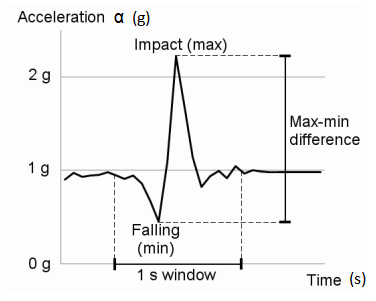
\includegraphics[scale=1]{images/KozinaImpact}
	\caption[Acceleration during impact]{Acceleration during impact according to Kozina et al. ~\cite{Kozina}}
	\label{fig:fallKozina}
\end{figure}
Taking into consideration the body orientation the single acceleration axis ($\alpha_x$, $\alpha_y$, $\alpha_z$) are essential to determine the person's body orientation. Assuming that the person is in a standing position (static posture), the x-acceleration ($\alpha_x$) corresponds to 1g (9.81$m/s^{2}$) and the other two axis ($\alpha_y$, $\alpha_z$) would be close to 0g (0$m/s^{2}$). This is a reference for a standing position. As soon as the person changes his posture, the gravitational force will act on one of the other two axis ($\alpha_y$, $\alpha_z$) and the x-acceleration will be 0g (0$m/s^{2}$). Combining this information with the acceleration magnitude (see Equation \ref{eq:acel}) the system is able to detect the fall and additionally determine the type of fall.

To ensure reliable fall detection, the system must be able to detect various types of falls. For this reason, the development of the fall detection prototype is also based on the creation of a test protocol covering different types of falls. The scientific papers by Li et al. \cite{Li2009} and Pannurat et al. \cite{Pannurat2014} were chosen as a reference, as they not only represent possible solutions for fall detection, but also offer a versatile overview of possible fall scenarios.

\section{Fall-detection system prototype}
\label{sec:fall-detectionPrototype}	

\subsection{Architecture}
\label{subsec:Architecture}	
The hardware architecture plays an important role in the development process to ensure the reliable functioning of the system. A first prototype was developed in this ongoing research which is introduced in \cite{LaBlunda.2016, LaBlunda.2016b}. In this paper an improved prototype will be introduced which. In order to guarantee a reliable functioning of the system, the hardware architecture plays an important role in the development process.  This paper presents an improved version of the prototype, which includes essential improvements that contribute to reliable operation of the system. Additionally, the improved hardware design meets the requirement for patient compliance. This aspect should be taken into consideration to provide a user friendly design which facilitates the freedom of movement for the user. As a safety critical system for medical purposes, a redundant hardware design should be provided to protect the system against a total system failure which would have severe consequences for the user in case of fall-events. Referring to J{\"a}ms{\"a} et al. \cite{jamsa2014fall} the best approach is to position the accelerometer near to the waist. Taking into consideration these aspects a wearable belt solution was developed which is based on a four sensor nodes BAN (see Figure \ref{fig:BanBelt}).
\begin{figure}[!ht]
	\centering
	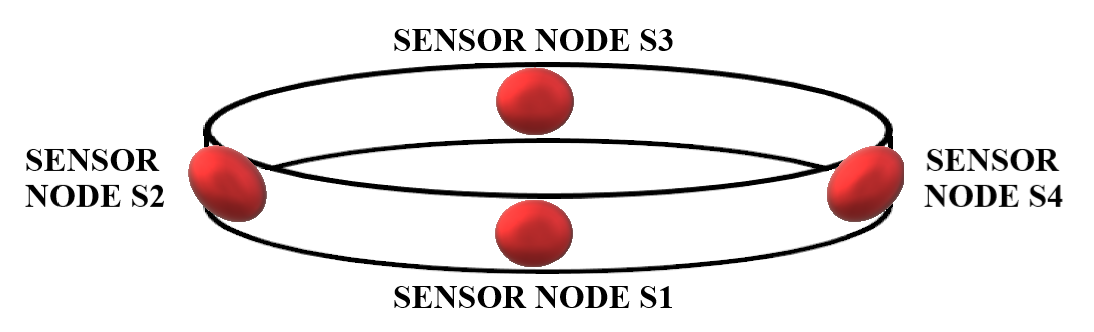
\includegraphics[scale=0.41]{images/belt}
	\caption[Four sensor nodes BAN - Belt]{Four sensor nodes BAN - Belt \cite{LaBlunda.2016, LaBlunda.2016b}}
	\label{fig:BanBelt}
\end{figure}

The four sensor nodes (S1 - S4) positioned on the belt are acting as peripherals and are continuously acquiring acceleration data which is sent via Bluetooth Low Energy to the smart phone (central device). The dataset consists of the following information: 
\begin{center}
 SensorID, X-Acceleration, Y-Acceleration, Z-Acceleration
\end{center}
\begin{itemize}
	\item \textbf{SensorID} $\rightarrow$ is used to identify to which sensor node the incoming dataset belongs to.
	\item \textbf{X-Acceleration} $\rightarrow$ represent the acceleration value in X-direction which the includes the unit m/$s^2$.
	\item \textbf{Y-Acceleration} $\rightarrow$ represent the acceleration value in Y-direction which the includes the unit m/$s^2$.
	\item \textbf{Z-Acceleration} $\rightarrow$ represent the acceleration value in Z-direction which the includes the unit m/$s^2$.
\end{itemize}
The central device receives the incoming sensor data which will be stored in separate text files to evaluate the event. 
The belt solution reflects the above criteria of a safety-critical systems. The proposed architecture (see Figure \ref{fig:BanBelt}) is based on a mirroring principle of the opposite sensor nodes which provide identical acceleration values, only with different signs. If a sensor node fails during operation, the opposite node can be used as a reference to ensure accurate evaluation of the event. Another positive consideration is the improvement of our system because of this hardware design. Considering the following scheme (see Figure \ref{fig:ReferenceScheme}) this fall-detection belt solution facilitates the recognition of different fall-event types. 

\begin{figure}[!ht]
	\centering
	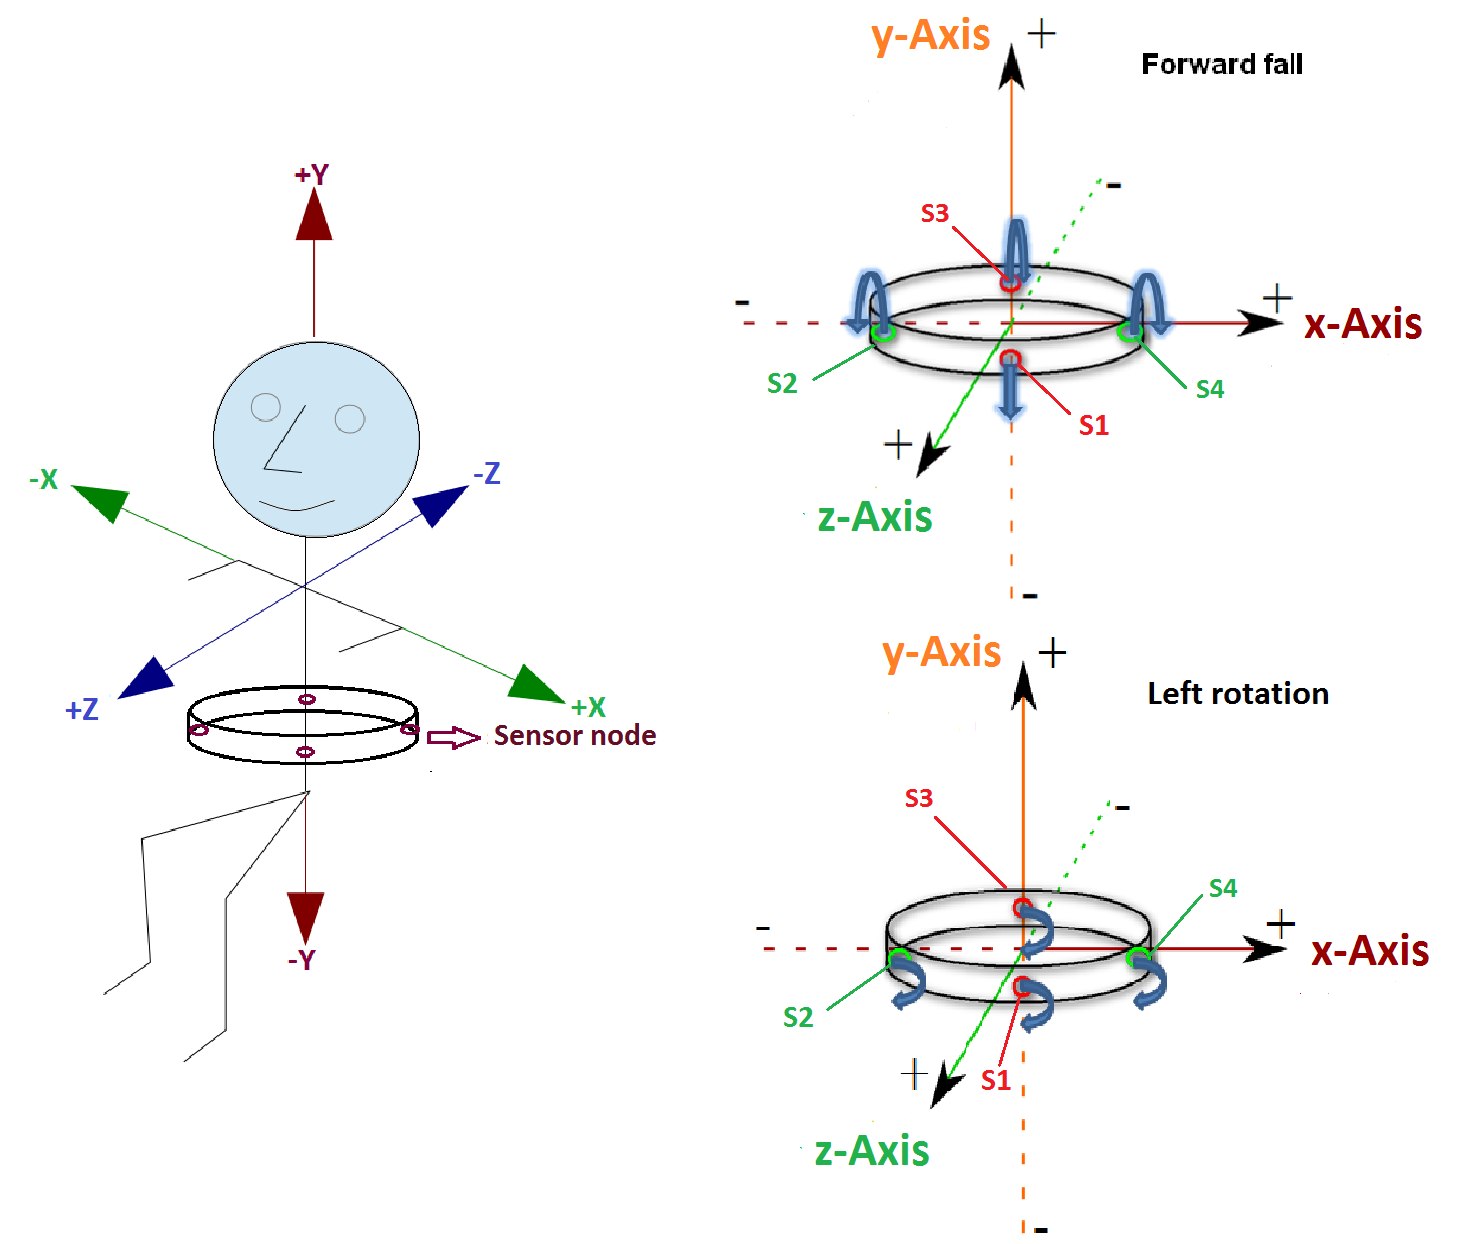
\includegraphics[scale=0.28]{images/axis}
	\caption[Three axis reference scheme]{Three axis reference scheme \cite{LaBlunda.2016,LuigiMasterThesis}}
	\label{fig:ReferenceScheme}
\end{figure}

The positioning of the nodes around the hip allows a more precise fall-characterization. Assuming that a person does a left rotation which leads to a frontal impact to the ground (forward fall), the single acceleration values ($\alpha_x$,  $\alpha_y$,  $\alpha_z$) could be used to determine the body's orientation and the acceleration magnitude (see Equation \ref*{eq:acel}) to detect the impact to the ground, as described in the previous section \ref{sec:background}. Taking into consideration the test protocol stated in section \ref{sec:background} typical fall-events (e.g. rolling out of the bed) in nursing homes and hospitals can be detected by this solution.


\subsection{Sensor fusion}
\label{subsec:sensorfusion}	
Analyzing the literature regarding fall detection, it was pointed out that the existing solutions show certain weaknesses in the reliable detection of falls. Considering Gjoreski et al. approach, his results with the fusion of physical sensors and the ECG sensor show a reliable fall detection. Especially the evaluation of the ECG signal leads to an essential improvement of the system's accuracy.  In \cite{Gjoreski2014} the ECG signal could be used to distinguish between different postures. The inclusion of medical parameters could even provide a fall prediction that would represent a significant progress in health care and prevent fatal injuries. Based on these results the proposed fall-detection belt  has been upgraded with a portable 3-channel ECG-sensor which provides an analog signal to the microcontroller. The successive illustration depicts the BAN structure of the update prototype architecture.
\begin{figure}[!ht]
	\centering
	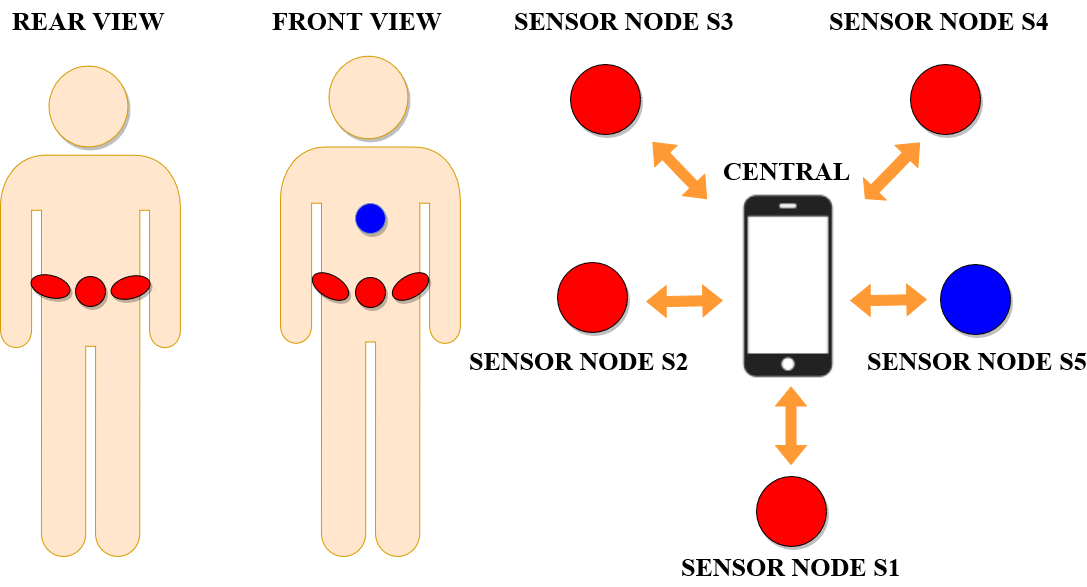
\includegraphics[scale=0.43]{images/ECG-BAN}
	\caption[ECG - BAN]{ECG - BAN}
	\label{fig:ECGBAN}
\end{figure}
The updated BAN includes four sensor nodes placed on the belt (S1 -S4) and an additional node on the chest (S5). These five nodes are acting as peripherals and they are continuously providing sensor data to the smart phone (central) via Bluetooth Low Energy. The sensor nodes S1 to S4 send the acceleration data and the ECG-sensor sends analog values (representation of ECG-signal) to the central device. Fusing these information the central device analyzes the events for possible fall-events.

Before the ECG-sensor can be fully integrated into the prototype, some tasks had be solved.  The first task to solve isA continuous recording of the ECG is required, even during the person's daily activities. The first task will be to facilitate a stable and continuous recording of the ECG, even during the person's daily activities. As the ECG-electrodes lose contact with the skin surface because of movement, this can lead to increased noise in the signal. Therefore, a solution for reliable ECG-recording have to be developed. The second task is to perform a validation of the ECG-sensor. For this purpose, the own ECG-measurements must be compared with measurements taken by a medically certified ECG-device, in order to guarantee the correctness of the ECG-values. Based on Gjoreski et al. \cite{Gjoreski2014} the ECG-signal is relevant to detect fall-events as mentioned in section \ref{sec:relatedwork}. Based on this, another task will be the determination of ECG patterns that provide relevant information for fall events.

The first test measurements with the ECG sensor confirmed the noisy and unstable ECG signal during movements. To ensure a stable and continuous signal during daily activities, an adjustable and flexible ECG-harness has been developed with prefabricated electrodes positioning and the ability to adapt to any body shape (see Fogure \ref{fig:ECGHarness}).
\begin{figure}[!ht]
	\centering
	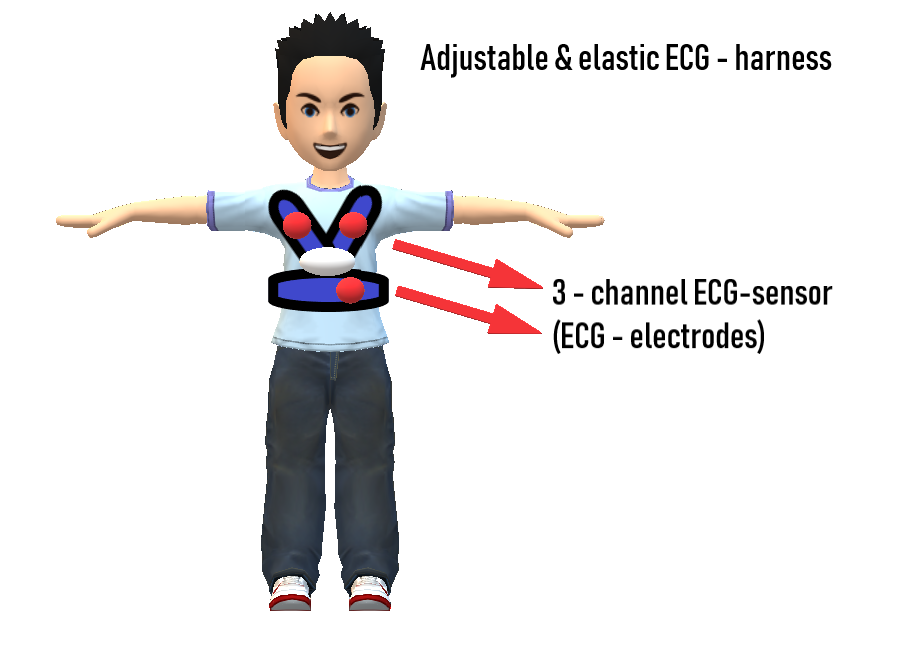
\includegraphics[scale=0.39]{images/ECG-Harness}
	\caption[ECG - Harness]{ECG - Harness}
	\label{fig:ECGHarness}
\end{figure}
After completing the development of the ECG-harness the measurements were repeated using the harness solution. A more stable signal resulted, especially during walking and the sitting procedure the stability of the ECG-signal was improved significantly. The artifacts in an ECG-signal which result during motion may be used as a recognition pattern for fall-events. After the positive results regarding the improved of the signal's stability validation test were conducted in a medical lab with the assistance of a physician. In the medical practice an ECG-device with 10 electrodes, but for wearable or emergency purposes (e.g. ambulance) a 3-Channel ECG-device is recommended because it provides less wiring and satisfy the aspect of patient compliance. Comparing the measurements taken in the medical lab with the ECG-measurements provided by our ECG-sensor the correct functionality of our sensor could be confirmed. The used sensor only differs in signal quality that includes noise and baseline shifting. The reasons for these distinctions in signal quality were explained by the supervising physician. Baseline wander (BW) disturbances are caused by variations in electrode-skin impedance, patient's movement and breathe during the ECG-measurements. Considering amyostasia disturbances the ECG-signal is affected by contraction of muscles near the heart which lead to noise in the signal. Muscle contraction is common for people which suffer from tremor or fearing the ECG-measurement and for disabled people. The certified medical devices have a integrated a filter which can be applied, to smooth the signal \cite{ECGNoise,DrNicoletteWagner}. 

\subsection{Generation of test-events}
Lorena's part  -->>> fall test events , highlight the test with synchronization problem

\subsection{Detected problems}

\section{Example application of STAMP as hazard analysis method}
\label{sec:STAMP}

\subsection{Introducing STAMP}
A fall-detection system is a safety critical system requiring certification according to a safety standard (e.g. IEC 60601-1) \cite{international2005medical}. To satisfy functional safety requirements it is fundamental to apply hazard analysis methods during development to analyze the behavior of the system in case of malfunctioning. This technique should be applied already in the early design phases to counteract developmental errors \cite{STAMPThesis}. In the following the classical hazard analysis method FMECA and the advanced method STAMP will be applied in some architectural parts of the fall-detection system for functional safety validation.

STAMP (System-Theoretic Accident Model and Processes) is a comprehensive hazard analysis method based on system theory. A major goal of this approach is to control or eliminate hazards. This approach proposed by Leveson \cite{leveson2011engineering} is used to identify probable accident causes that are categorized as follows:
\begin{itemize}
	\item Accidents based on hardware and software component failure
	\item Unsafe interactions among components
	\item Complex human machine interfaces and human error models
	\item Erros in system design
	\item Faulty requirements
\end{itemize}  
STAMP treats accidents as a control problem. To prevent accidents safety constraints derived from system safety requirements must be enforced inside the different system hierarchy levels. If the given safety constraints are violated accidents may occur. Checking the enforcement of safety constraints leads to an additional layer of system testing.

\subsection{STAMP - Hazard analysis}
STAMP begins on the system level and proceeds top down into the system hierarchy. To apply STAMP the following steps must be followed:
\begin{itemize}
	\item \textbf{Definition of accidents:} Person has fallen and the fall was not detected by the system.
	\item \textbf{Definition of hazards:} Data from 1 to 4 sensors of the belt are not sufficiently correlated in time (synchronization error).
	\item \textbf{Definition of safety requirements \& constraints:} The safety requirements and constraints are based on the hazard which causes the accident. A top level safety requirement is the real-time detection of fall-events. The timestamps of all four nodes must be synchronized. If constraints are violated system migrates to unsafe or hazardous state.
\end{itemize}
\section{Conclusion \& Future work}
\label{sec:conclusion}

\section{Bibliography styles}

There are various bibliography styles available. You can select the style of your choice in the preamble of this document. These styles are Elsevier styles based on standard styles like Harvard and Vancouver. Please use Bib\TeX\ to generate your bibliography and include DOIs whenever available.

Here are two sample references: \cite{Feynman1963118,Dirac1953888}.

\section*{References}

\bibliography{mybibfile}

\end{document}